
\documentclass[12pt]{article}


\usepackage{indentfirst}
\usepackage{graphicx}
\usepackage[margin=1.3in, top=1.4in]{geometry}
\usepackage[section]{placeins}
\usepackage{booktabs}
\usepackage{tabularx} 
\usepackage{tabulary}
\usepackage{cutwin}
\usepackage{caption}
\usepackage{lipsum}
\usepackage{wrapfig}
\usepackage[utf8]{inputenc}
\usepackage[T1]{fontenc}
\usepackage{color}
\usepackage{eurosym}
\usepackage{glossaries}
\usepackage{subcaption}
\usepackage{amsmath}
\usepackage{float}
\usepackage{listings}
\usepackage{color}
\usepackage[table,xcdraw]{xcolor}
\definecolor{mygreen}{rgb}{0,0.6,0}
\definecolor{mygray}{rgb}{0.5,0.5,0.5}
\definecolor{mymauve}{rgb}{0.58,0,0.82}
% Define Language
\lstdefinelanguage{EL}
{
	% list of keywords
	morekeywords={language, 
		annotation,
		interface,
		service, 
		services, 
		reference, 
		references, 
		properties, 
		int, 
		float, 
		string, 
		bool, 
		subcomponents, 
		component, 
		bind, 
		to, 
		promote, 
		as,
		import,
		compile }, 
	sensitive=false, % keywords are not case-sensitive
	morecomment=[l]{//}, % l is for line comment
	morecomment=[s]{/*}{*/}, % s is for start and end delimiter
	morestring=[b]" % defines that strings are enclosed in double quotes
}
% Set Language
\lstset{
	%language={EL},
	aboveskip=2\bigskipamount,
	backgroundcolor=\color{white}, % choose the background color; you must add \usepackage{color} or \usepackage{xcolor}
	basicstyle=\scriptsize, % the size of the fonts that are used for the code
	breakatwhitespace=false, % sets if automatic breaks should only happen at whitespace
	breaklines=true, % sets automatic line breaking
	captionpos=b, % sets the caption-position to bottom
	commentstyle=\color{mygreen}, % comment style
	deletekeywords={...}, % if you want to delete keywords from the given language
	escapeinside={\%*}{*)}, % if you want to add LaTeX within your code
	extendedchars=true, % lets you use non-ASCII characters; for 8-bits encodings only, does not work with UTF-8
	frame=lines, % adds a frame around the code
	keepspaces=true, % keeps spaces in text, useful for keeping indentation of code (possibly needs columns=flexible)
	keywordstyle=\color{blue}, % keyword style
	% otherkeywords={*,language, interface,
	% service, services, reference, references, properties, int, float, string, bool, subcomponents, component, bind, to, promote, as,import,compile, ...}, % if you want to add more keywords to the set
	numbers=none, % where to put the line-numbers; possible values are (none, left, right)
	numbersep=5pt, % how far the line-numbers are from the code
	numberstyle=\tiny\color{mygray}, % the style that is used for the line-numbers
	rulecolor=\color{black}, % if not set, the frame-color may be changed on line-breaks within not-black text (e.g. comments (green here))
	showspaces=false, % show spaces everywhere adding particular underscores; it overrides 'showstringspaces'
	showstringspaces=false, % underline spaces within strings only
	showtabs=false, % show tabs within strings adding particular underscores
	stepnumber=2, % the step between two line-numbers. If it's 1, each line will be numbered
	stringstyle=\color{mymauve}, % string literal style
	tabsize=2, % sets default tabsize to 2 spaces
	title=\lstname, % show the filename of files included with \lstinputlisting; also try caption instead of title
	%xleftmargin=20.0pt,
	%xrightmargin=20.0pt
}
\definecolor{mygreen}{rgb}{0,0.6,0}
\definecolor{mygray}{rgb}{0.5,0.5,0.5}
\definecolor{mymauve}{rgb}{0.58,0,0.82}
\lstset{ %
  backgroundcolor=\color{white},   % choose the background color; you must add \usepackage{color} or \usepackage{xcolor}
  basicstyle=\scriptsize,        % the size of the fonts that are used for the code
  breakatwhitespace=false,         % sets if automatic breaks should only happen at whitespace
  breaklines=true,                 % sets automatic line breaking
  captionpos=b,                    % sets the caption-position to bottom
  commentstyle=\color{mygreen},    % comment style
  escapeinside={@*}{@},          % if you want to add LaTeX within your code
  extendedchars=true,              % lets you use non-ASCII characters; for 8-bits encodings only, does not work with UTF-8
  frame={bottom and top},	                   % adds a frame around the code
  keepspaces=true,                 % keeps spaces in text, useful for keeping indentation of code (possibly needs columns=flexible)
  keywordstyle=\color{blue},       % keyword style
  language=c++,                      % the language of the code
  otherkeywords={*,...},           % if you want to add more keywords to the set
  numbers=none,                    % where to put the line-numbers; possible values are (none, left, right)
  numbersep=5pt,                   % how far the line-numbers are from the code
  numberstyle=\tiny\color{mygray}, % the style that is used for the line-numbers
  rulecolor=\color{black},         % if not set, the frame-color may be changed on line-breaks within not-black text (e.g. comments (green here))
  showspaces=false,                % show spaces everywhere adding particular underscores; it overrides 'showstringspaces'
  showstringspaces=false,          % underline spaces within strings only
  showtabs=false,                  % show tabs within strings adding particular underscores
  stepnumber=2,                    % the step between two line-numbers. If it's 1, each line will be numbered
  stringstyle=\color{mymauve},     % string literal style
  tabsize=2,	                   % sets default tabsize to 2 spaces
  title=\lstname,                   % show the filename of files included with \lstinputlisting; also try caption instead of title
  aboveskip=1.5em,
  belowskip=1em
}

%%%%%%%%%%%%%%%%%%%%%%%%%%%%%%%%%%
%subsubsubsection
%%%%%%%%%%%%%%%%%%%%%%%%%%%%%%%%%%
\usepackage{titlesec}
%\usepackage{hyperref}
\usepackage[hidelinks]{hyperref}

\titleclass{\subsubsubsection}{straight}[\subsection]
\newcounter{subsubsubsection}[subsubsection]
\renewcommand\thesubsubsubsection{\thesubsubsection.\arabic{subsubsubsection}}
\renewcommand\theparagraph{\thesubsubsubsection.\arabic{paragraph}} % optional; useful if paragraphs are to be numbered
\titleformat{\subsubsubsection}
  {\normalfont\normalsize\bfseries}{\thesubsubsubsection}{1em}{}
\titlespacing*{\subsubsubsection}
{0pt}{3.25ex plus 1ex minus .2ex}{1.5ex plus .2ex}
\makeatletter
\renewcommand\paragraph{\@startsection{paragraph}{5}{\z@}%
  {3.25ex \@plus1ex \@minus.2ex}%
  {-1em}%
  {\normalfont\normalsize\bfseries}}
\renewcommand\subparagraph{\@startsection{subparagraph}{6}{\parindent}%
  {3.25ex \@plus1ex \@minus .2ex}%
  {-1em}%
  {\normalfont\normalsize\bfseries}}
\def\toclevel@subsubsubsection{4}
\def\toclevel@paragraph{5}
\def\toclevel@paragraph{6}
\def\l@subsubsubsection{\@dottedtocline{4}{7em}{4em}}
\def\l@paragraph{\@dottedtocline{5}{10em}{5em}}
\def\l@subparagraph{\@dottedtocline{6}{14em}{6em}}
\makeatother
\setcounter{secnumdepth}{4}
\setcounter{tocdepth}{4}

\newenvironment{abbreviations}{\begin{list}{}{\renewcommand{\makelabel}{\abbrlabel}}}{\end{list}}
\newcommand{\abbrlabel}[1]{\makebox[3cm][l]{\textbf{#1}\ \dotfill}}
%%%%%%%%%%%%%%%%%%%%%%%%%%%%%%%%%%%%%%%%%%%%%%%

\newenvironment{EBNF}
{\captionsetup{type=lstlisting}}
{}

%----------------------------------------------------------------------------------------
%	TITLE
%----------------------------------------------------------------------------------------
\begin{document}

\begin{titlepage}
\newcommand{\HRule}{\rule{\linewidth}{0.5mm}} % Defines a new command for the horizontal lines, change thickness here
\center % Center everything on the page

%----------------------------------------------------------------------------------------
%	HEADING SECTIONS
%----------------------------------------------------------------------------------------

%\textsc{\LARGE FINAL REPORT}\\[1.0cm] % Major heading such as course name
%\textsc{\Large Project II}\\[0.5cm] % Minor heading such as course title
\textsc{\large Embedded Systems Research Group}\\[0.5cm] % Minor heading such as course title

%----------------------------------------------------------------------------------------
%	TITLE SECTION
%----------------------------------------------------------------------------------------

\HRule \\[1.2cm]
{ \Huge \bfseries 
Weightlifting}\\[1.0cm] % Title of your document 
\HRule \\[3.0cm]
 
%----------------------------------------------------------------------------------------
%	AUTHOR SECTION
%----------------------------------------------------------------------------------------
% Your name
\begin{minipage}{0.4\textwidth}
\begin{flushleft} \large
\emph{Authors:}\\
Class 2016/2017   \\
\end{flushleft}
\end{minipage}
~
\begin{minipage}{0.4\textwidth}
\begin{flushright} \large
 \emph{Advisor:} \\
Adriano \textsc{Tavares} \\ % Supervisor's Name
\end{flushright}
\end{minipage}\\[2cm]

%----------------------------------------------------------------------------------------
%	LOGO SECTION
%----------------------------------------------------------------------------------------
\noindent\begin{minipage}{0.2\textwidth}
\includegraphics[width=\linewidth]{Images/UMLogo}\\ [0.5cm] 
\end{minipage}%
\hfill%



{ \large \bfseries 
Universidade do Minho}\\[0.5cm] 

%----------------------------------------------------------------------------------------
%	DATE SECTION
%----------------------------------------------------------------------------------------
{\large \today}\\[3cm] % Date, change the \today to a set date if you want to be precise
\vfill % Fill the rest of the page with whitespace

\end{titlepage}



%----------------------------------------------------------------------------------------
% Table of Contents
%----------------------------------------------------------------------------------------
\pagenumbering{roman}
\renewcommand{\listfigurename}{Contents}
\tableofcontents
\newpage
%----------------------------------------------------------------------------------------
% Table of Figures
%----------------------------------------------------------------------------------------
%\renewcommand{\listfigurename}{Figures}
%\listoffigures
%\newpage
%----------------------------------------------------------------------------------------
% Table of Tables
%----------------------------------------------------------------------------------------
%\renewcommand{\listtablename}{Tables}
%\listoftables

%----------------------------------------------------------------------------------------
% Table of Listings
%----------------------------------------------------------------------------------------
%\lstlistoflistings
%\newpage

%----------------------------------------------------------------------------------------
% Glossaries
%----------------------------------------------------------------------------------------
%\newglossaryentry{utc}{name=UTC, description={Coordinated Universal Time}} %\gls{utc}
%\printglossaries

%----------------------------------------------------------------------------------------
% Introduction
%----------------------------------------------------------------------------------------
\newpage
\pagenumbering{arabic}
\section{Introduction}

\input{texts/Introduction}

%----------------------------------------------------------------------------------------
% Theoretical Concepts
%----------------------------------------------------------------------------------------
\newpage
\section{Design Methodology}
The methodology employed in this study consists of three phases composed of several activities.
In the first phase, the ontology design and development are carried out following a set of steps.
In the second phase, ontology validation is accomplished by an iterative refining process.
In the third phase, the ontology is implemented in a software application using an API for easier integration.

\subsection{Phase I - Design and Development} \label{phasesChapter}

The first phase is carried out using an ontology-based platform such as Protégé and OWL for the ontology representation.

The first step consists in the definition of the ontology scope by identifying the domain of the ontology, its purpose and functionalities and the end-users.

In the second step should be considered the possibility of reusing existing ontologies instead of developing one from scratch.
Many ontologies may already be available and can be easily imported into an ontology-based platform.

In the third step is performed the identification of the key concepts of the ontology being developed.
This task can be done following a top-down, bottom-up or middle-out approach in the elicitation of the different concepts.

In the forth step are identified concept to properties relationships.
This is carried out by defining and developing properties that represent relationships between one or more concepts.

In the fifth step are identified concept to instance relationships.
This step is similar to the last, but moves one step further into the lower-level, more detailed and complex relationships, since an instance is a specific realisation of a concept.

\subsection{Phase II - Validation}
 
The second phase encompasses various validation tasks that should be executed in a systematic approach.
Employment of metrics for ontology validation.
The usage of reasoners for correct verification of consistency of the developed ontology or ontologies.
Assessment of functional and non-functional requirements.

\subsection{Phase III - Implementation}

The last phase consists in the implementation of the developed ontology.
A suitable ontology API should be selected according to the appropriate application being developed that will ease the integration process of both artifacts.



	
\newpage
%----------------------------------------------------------------------------------------% 
% Ontology Design and Development
%----------------------------------------------------------------------------------------
\section{Design and Development}

\subsection{Step 1}
Taking into account the steps mentioned in chapter \ref{phasesChapter} for the design and development of a product ontology, the first step that should be performed is the definition of the ontology's domain and use case scenarios. This is about capturing the necessary knowledge for the framework development.
\par The domain defines the knowledge area that the structure and vocabulary of an ontology is designed for.
\par The use case scenarios are defined in order to acquire the main objectives for the ontology, the set of questions that ontology should answer, the users that interact with it, and the questions related with its maintainability.
\par Sanya and Shehab \cite{AeroArticle} define these terms through four simple questions that should be answered in this phase:
\begin{enumerate}
\item What is the domain?
\item What can the ontology be used for?
\item What questions should the ontology answer?
\item Who will use and maintain it?
\end{enumerate}

\par The ontology developed by Hugo Dias \cite{HugoThesis} in his thesis refers to the biomechanical domain in Olympic Weightlifting training sessions.
This ontology is used to improve the posture of weightlifting athletes, and with this improve their performance and prevent serious injuries. It can also be used to see the progress of an athlete and help manager teams in the training sessions.
It should answer if the athlete, during a training session, performed the weightlifting properly. If not, it should mention what was wrong and what body position should be changed in order to perform the exercise properly.
The developed ontology will be used by athletes and their manager teams. It can be assumed that it will not have any type of maintenance since there's no information about that issue in Hugo Dias' \cite{HugoThesis} thesis. 
\par Table \ref{tab:1st} summarizes all the information that should be collected during this phase. 

\begin{table}[H]
\centering
\caption{Step 1 - Defining the domain and use case scenarios.}
\label{tab:1st}
\begin{tabular}{p{7cm} p{7cm}}
\hline
What is the domain?                        & \begin{tabular}[c]{p{7cm}} - Biomechanical knowledge in Olympic Weightlifting  \end{tabular}
\\ \hline
What can the ontology be used for?         & \begin{tabular}[c]{p{7cm}}-
 Understanding the failures of athletes \\ - Improving the posture of athletes\\ - Preventing injuries in the trains\\ - Improving the overall performance\\ - Verify the athletes' progress\\  - Help managers and athletes\end{tabular} \\ \hline
What questions should the ontology answer? & \begin{tabular}[c]{p{7cm}}- The athlete performed the weightlifting correctly?\\ - There was something wrong with the athlete's posture?\end{tabular}                                                                                                                                                                   \\ \hline
Who will use and maintain it?              & \begin{tabular}[c]{p{7cm}}- It will be used by athletes and their managers teams.\\ - It won't be maintained.\end{tabular}                                                                                                                                                                        \\ \hline
\end{tabular}
\end{table}

\subsection{Step 2}
\par It's very important to search ontologies already done by someone else before starting one from scratch. We couldn't find an ontology that replaces the one developed by Hugo Dias in his thesis, because it is very specific to the weightlifting sport.
\par However, since this ontology is supposed to describe the Olympic weightlifting, it's development could be started by an Olympic ontology. 
\par We found in \url{http://swat.cse.lehigh.edu/resources/onto/olympics.owl}  a good source to extend for Hugo's ontology particular domain. 

\subsection{Step 3}
The third step on ontology design consists in defining the ontology concepts and its UML representation. Concepts are OWL classes that describe a specific domain.

The domain of the ontology is weightlifting and after a quick study the concepts were found: the \textbf{Athlete} class represents the athlete's profile and its properties such as name, age and weight, the \textbf{Barbell} class represents the piece of equipment that is lifted during the exercise and the \textbf{Exercise} class represents the exercise itself. This last concept is divided in other two that represent different competitions of the Olympic weightlifting: the \textbf{Snatch} and \textbf{Clean and Jerk}.

The concepts have different relationships between them, which can be described as:
\begin{itemize}
	\item Athlete \textbf{practices} Exercise, 
	\item Exercise \textbf{is practiced by} Athlete,
	\item Athlete \textbf{lifts} Barbell,
	\item Barbell \textbf{is lifted by} Athlete,
	\item Exercise \textbf{has} Barbell,
	\item Barbell \textbf{is part of} Exercise.
\end{itemize}

Figure \ref{UML} represents the high level UML representation of this Ontology with all the concepts and correspondent relationships. 

\begin{figure}[H]
	\includegraphics[width=0.9\linewidth]{Images/step3_UML.png}
	\caption{UML representation.}
	\label{UML}
\end{figure}




\subsection{Step 4 - Identify concept to properties relationships}
This phase has the purpose of identification of the properties developed for the ontology that allow the \textbf{relationship} between one or more concepts.

For the Weightlifting ontology, two kind of OWL properties were developed: \textbf{Object} and \textbf{Data} properties. 

Object properties were developed to define explicit relationships between one or more concepts. Object properties such as 'practices', 'lifts', 'has', 'isPracticedby', 'isliftedBy' and 'isPartOf', were developed in order to make possible the establishment of relationships between one or more concepts. As already said, each property establishes relationships and their descriptions are presented below: 

\begin{itemize}  
	\item Object property 'practices' relates Athlete class to Exercise class and assures that the Athlete always practices an exercise.
	\item Object property 'lifts' relates Athlete class and Barbell class, meaning that an athlete lifts a barbell.
	\item Object property 'has' relates Exercise class and Barbell class, meaning that an weightlifting exercise has a barbell.
	\item Object property 'isPracticedby' is the inverse property of 'practices'.
	\item Object property 'isliftedBy' is the inverse property of 'lifts'.
	\item Object property 'isPartOf' is the inverse property of 'has'.
\end{itemize}

Data properties were developed to define explicit relationships between concepts and data values. These properties were developed to accommodate some cases where three-dimensional variables are necessary to measure specific lifting positions, during the athlete exercise. Data properties such as the knee or ankle three-dimensional position along the athlete lifting series are example of properties developed in order to make possible the establishment of relationships between one or more concepts.

\subsection{Step 5}
In this step it is necessary to identify concept to instance relationships. An instance is a specific realization of a concept. Each realized specification of a concept is defined as the process of instantiation. Defining relationships between instances and concepts is often not employed in ontology development as many ontology development efforts focuses on high-level concept to concept relationships. Relationships between instances and concepts enable the definition of complex relationships within the ontology domain. 
    
As mentioned before, an ontology does not need to have instances and the relationships between instances and concepts do not need to be pointed out. This ontology is a perfect example, as it does not possess any instance and so there are no concept to instance relationships. 


\newpage
%----------------------------------------------------------------------------------------
% Ontology Validation
%---------------------------------------------------------------------------------------
\section{Validation}
\input{texts/OntologyValidation}

\subsection{Reasoners}

This section provides an overview and comparison of two reasoners, Pellet and Hermit, taking into account the final application and ontology. The Fact++ and RacePro reasoners are also included in the comparison to provide an additional reference for comparison.
Although the target ontology's characteristics are not yet known, the analysis performed on the specified reasoners is based on the work performed by \cite{Dentler2011} and \cite{Bock2008}, which consist on the creation of complete benchmarks based on several important characteristics, such as practicability and performance.

A reasoner is a program that infers logical consequences from a list of explicit asserted facts or axioms and typically provides automated support for reasoning tasks such as classification, debugging and querying.

The reasoner presented are: HermiT \cite{1_hermitreasoner}, Pellet \cite{2_stardog-union/pellet_2016}, Fact++ \cite{3_fact++reasoner} and RacerPro \cite{4_racerpro_2016}. This set has several common characteristics which seem to be essential to the final application. In terms of practical usability, they are accessible through the OWL API and can be plugged into Protege, except RacerPro. Since they possess the same interfaces, they can be interchanged providing development flexibility, allowing to easily compare them. Also all the referred reasoners implement tableux algorithms which guarantees soundness - all the inferred statements a correct - and completeness - how many correct statements are inferred. A small description of each reasoner follows:

\begin{itemize}
\item \textbf{Hermit} - This Java-based OWL reasoner is based on a new tableau reasoning algorithm. It can be integrated into Protege e and Java applications using the OWL API.
\item \textbf{Pellet} - This is an open-source, Java-based OWL DL reasoning engine that supports a majority of the constructs of OWL, including those introduced in OWL 2. Pellet is developed and commercially supported by Clark and Parsia.
\item \textbf{FaCT++} - An open-source reasoner, which implemented in C++, supports large subset of OWL DL and is based on optimized tableaux algorithms.
\item \textbf{RacerPro} (Renamed ABox and Concept Expression
Reasoner, Racer Systems) supports a large subset of OWL DL. It is implemented in the Common Lisp programming language.
\end{itemize}

\subsubsection{Performance Comparison}

The developed performance benchmark in \cite{Dentler2011} uses two typical reasoner tasks, consistency checking and classification. Consistency checking verifies whether there exists a relational structure that satisfies all axioms in the given ontology, that is, if there are no contradictory statements in the ontology. Classification is the computation of the concept hierarchy and relationship. This is often used as the main performance indicator. The ontology should be checked for consistency and classified regularly, with every modification made to it. 

Using several well established ontologies in the biomedical field, \cite{Dentler2011} evaluates the performance of several reasoners (including HermiT, Pellet and Fact++) according to the previously mentioned reasoner tasks, among other characteristics. This ontologies have the same OWL profile but different sizes in order to evaluate a possible trade off between ontologies' complexity and reasoner's performance. The ontologies used were GO, NCI and SNOMED CT which are listed in ascendant order of size in tables \ref{tab:1} and \ref{tab:2}. According to the data provided in \cite{Dentler2011} present in table \ref{tab:1}, all tested reasoners succeeded in classifying SNOMED CT and the Fact++ was the only reasoner who classified the NCI faster than the GO ontology. HermiT reasoner had the worst performance when classifying the SNOMED CT ontology taking up to two hours to perform the task.

\begin{table}[]
\centering
\begin{tabular}{|l|l|l|l|}
\hline
      &  HermiT    &  Pellet     &  Fact++    \\ \hline
GO    &    6.48    &  3.41       &  20.75     \\ \hline
NCI   &   11.75    &  14.84      &  11.10     \\ \hline
S CT  &  6,793.76  &  1,345.65   &  700.87    \\ \hline
\end{tabular}
\caption{Reasoner classification performance comparison in \cite{Dentler2011} (s).}
\label{tab:1}
\end{table}

Consistency checking performance per reasoner is depicted in table \ref{tab:1}. The recorded times are mostly insignificant except for the SNOMED CT ontology where HermiT outperforms the other reasoners by a large margin.

\begin{table}[]
\centering
\begin{tabular}{|l|l|l|l|}
\hline
      &  HermiT  &  Pellet   &  Fact++ \\ \hline
GO    &    0.00  &  0.27     &  0.36   \\ \hline
NCI   &    0.00  &  0.38     &  0.71   \\ \hline
S CT  &    0.00  &  16.78    &  15.3   \\ \hline
\end{tabular}
\caption{Reasoner consistency check performance comparison in \cite{Dentler2011} (s).}
\label{tab:2}
\end{table}

It should be noted that, independently of the used reasoner, the performance decreases with increasing ontology size and complexity.

In \cite{Bock2008} a different kind of analysis is performed. Reasoners are compared according to their Load and Response Time.
Load Time is the time required to perform some important preparation before classification, consistency check and querying ontologies. Response Time starts with querying execution and ends when all the results are stored in a local variable. 
In the tests by \cite{Dentler2011}, the tested ontologies were implemented according to the same OWL profile. The study by \cite{Bock2008} takes a diffrent approach and tests ontologies implemented in different OWL profiles, which appear in ascending expressiveness order in tables \ref{tab:3} and \ref{tab:4}. 

\begin{table}[]
\centering
\begin{tabular}{|l|l|l|l|}
\hline
          &   HermiT  &  Pellet & RacerPro\\ \hline
VICODI    &    0.889  &  0.563  & 0.110   \\ \hline
SWRC      &    0.776  &  0.518  & 0.092   \\ \hline
LUBM      &    0.708  &  0.404  & 0.072   \\ \hline
WINE      &    1.090  &  0.835  & 0.0168  \\ \hline
\end{tabular}
\caption{Load time performance comparison in \cite{Bock2008} (s).}
\label{tab:3}
\end{table}

\begin{table}[]
\centering
\begin{tabular}{|l|l|l|l|}
\hline
          &  HermiT  &  Pellet  & RacerPro \\ \hline
VICODI    &    0.180  &  1.145  & 0.080 \\ \hline
SWRC      &    0.046  &  0.346  & 0.056 \\ \hline
LUBM      &    0.046  &  0.253  & 0.365 \\ \hline
WINE      &    0.465  &  9.252  & 0.607 \\ \hline
\end{tabular}
  \caption{Response time performance comparison in \cite{Bock2008} (s).}
\label{tab:4}
\end{table}

By looking at the above tables it is clear that, although Pellet and RacePro show better performance at load time, they also shows significant less performance than HermiT when queries are executed, especially for higher complexity ontologies. This comparison depends on whether the application frequently operates on preloaded ontologies or has to re-loaded them at each classification, since in the former case load times become irrelevant. 


\subsubsection{Final Thoughts}

Based on the literature, two benchmarks and the respective results were analyzed to select the reasoners that best fit application's requirements. Between Pellet and HermiT, at first sight the HermiT reasoner shows a better performance than Pellet.  Unfortunately, a decision can not be made on a specific reasoner since application requirements are not yet known. Another important point for reasoner selection are the target ontology's characteristics, such as size or expressiveness, which are also unknown. 

Since reasoner performance is largely dependent on ontology and application characteristics, when developing an ontology and its application, the various reasoners should be tested regularly in order to decide which one bests suits the system requirements. Because of this, an important characteristic of the selected reasoners is that they should provide an interface via a common ontology API, such as the OWL API, and have a Protege plugin, which will allow to easily interchange them at development time for performance testing. 


\subsection{Ontology Requirements}
Regarding the project requirements, the vast majority of them referred to the application instead of the ontology. The presented functional requirements for the application concern mainly the user interaction and the non-functional ones described the response time and friendliness of the application. These requirements have been met when the project was over.

Concerning the presented ontology requirements, the first one detailed how the system must apply the rules and query the ontology, and the second one assumed that the system should give some recommendations to the user, from the rules inferred. Both of these requirements were almost fulfilled given the ontology limitations. One of the main issues found was the lack of a range of accepted values in the rules that infer if the move was correct. This solution would have improved the system reliability on the results obtained.

The ontology structure developed is very minimalistic, which allows its integration in different projects within the area of weightlifting but not without any modifications. The ontology simplistic nature is also its downside, failing to detail some parts of its domain like muscles or specific parts of the body.

\subsection{Consistency Checking}
\input{texts/ConsistencyChecking}

\newpage
%----------------------------------------------------------------------------------------
% Ontology Implementation
%---------------------------------------------------------------------------------------
\section{Implementation}
\input{texts/OntologyImplementation}

\subsection{Ontology APIs}
An ontology API provides a set of tools to interact with ontologies from a specific programming language. There are some key features to have in mind when choosing these APIs (e.g., purpose, flexibility, application's programming language, ontology representation format). When the purpose of the interface includes reasoning, it becomes important to include Reasoner Compatibility in the desired features.

\subsubsection{Ontology Data Model Manipulation API}

In this section, the desired purpose is to provide methods to load an OWL file and edit its ontology model. The interface must be implemented in JAVA. The following APIs will be evaluated considering the previously mentioned restrictions:
\begin{itemize}
	\item OWL API
	\item Jena API
	\item Protégé-OWL API
\end{itemize}

The OWL API is an Open Source Java API for creating, manipulating and serializing OWL Ontologies. It is able to read numerous ontology formats apart from OWL and OWL2, such as RDF, Turtle, KRSS and OBO. It has one of the easiest JAVA programming interfaces. The user can load and save ontologies, create or delete entities, interact with reasoners, among other functionalities. Two reasoner implementations are available --- Pellet and FaCT\texttt{++}. It supports SWRL rules but not SPARQL queries. Since SPARQL is an RDF query language, this means that the interface is not RDF-friendly.

Jena API, on the other side, covers RDF manipulation at its fullest. This means that it is extremely flexible since it can be used to create OWL constructs, axioms and run inferences. Unlike the OWL API, it is capable of running SPARQL queries. The provided interface is also written in JAVA but it is slightly more complex. This API already includes various reasoners to cope with different tasks, such as transitive and reflexive properties solving; RDFS, OWL and generic rule solving.

Finally, the Protégé-OWL API is an extension of the core Protégé API. It stands as an open-source JAVA tool. To load RDF ontologies it uses ARP, which is the parsing subsystem in Jena to handle the RDF/XML syntax. It is possible to convert a Protégé OWLModel into a Jena OntModel. This close relationship with Jena doesn't end here since it reuses species validation, datatype handling services and a graph interface from Jena. This API can be used  to manage all aspects of the Protégé internal representation. This kind of flexibility comes at the expense of low-level and less user-friendly methods.

Protégé-OWL was the chosen API due to its scarce limitations and large available documentation.


\subsubsection{SQWRL API}

Protégé provides SWRLAPI, which is a very useful interface for working with the OWL-based SWRL rule and SQWRL query languages. It includes graphical tools for editing and executing rules and queries.  

When a query is executed, the API uses a rule engine to run all SWRL rules. It works as an inference agent to gather all the knowledge from the rules, providing the query engine with supplementary information. The API can, however, run a standalone SQWRL query method without running SWRL rules.


\subsubsection{Reasoning API}

Another important interface is the Protege-OWL Reasoner API. It provides programmatic access to a direct or a DIG-compliant reasoner. It implements methods for consistency checking, classification of an ontology as well as methods for getting the inferred information for a particular OWL entity. 

One of the most documented reasoners to work with this API is Pellet. This reasoner can access the ontology through a Jena model or a Protege-OWL model. As mentioned earlier, the close relationship between Protégé and Jena makes it possible to convert an OWLModel into an OntModel. Once converted, the user can then create a ProtegeReasoner class instance and start the inferring process.



\subsection{Integration}
As stated previously, it is necessary to integrate the developed ontology with a Java application.
The developed Java application will be used to manage athletes' training sessions data and provide feedback on their posture.
The ontology will be used to infer the correct execution of a weightlifting exercise based on the data received from training.

Displayed in Figure~\ref{fig:ont_int} is part of the application behavior.
Starting with a click event, an XML parsing process is initiated to convert rules into an SQWRL query format.
After that, is established a connection to an SQL database to retrieve the athlete's training data.
Then is performed a conversion of the ontology OWLModel to an OntModel for it to be used with the SQWRL query engine.
In the generated OntModel is created an individual to hold the athlete's training session data that will be used for the inference process.
Because this is done in a "temporary" model, none of these actions will have any effect on the developed ontology.
Finally, the inference process takes place with the execution of each query through the Query Engine.
In the end of this process the results are displayed, telling the athlete which parts of the exercise were well done and not well done.

\begin{figure}[h]
	\centering
		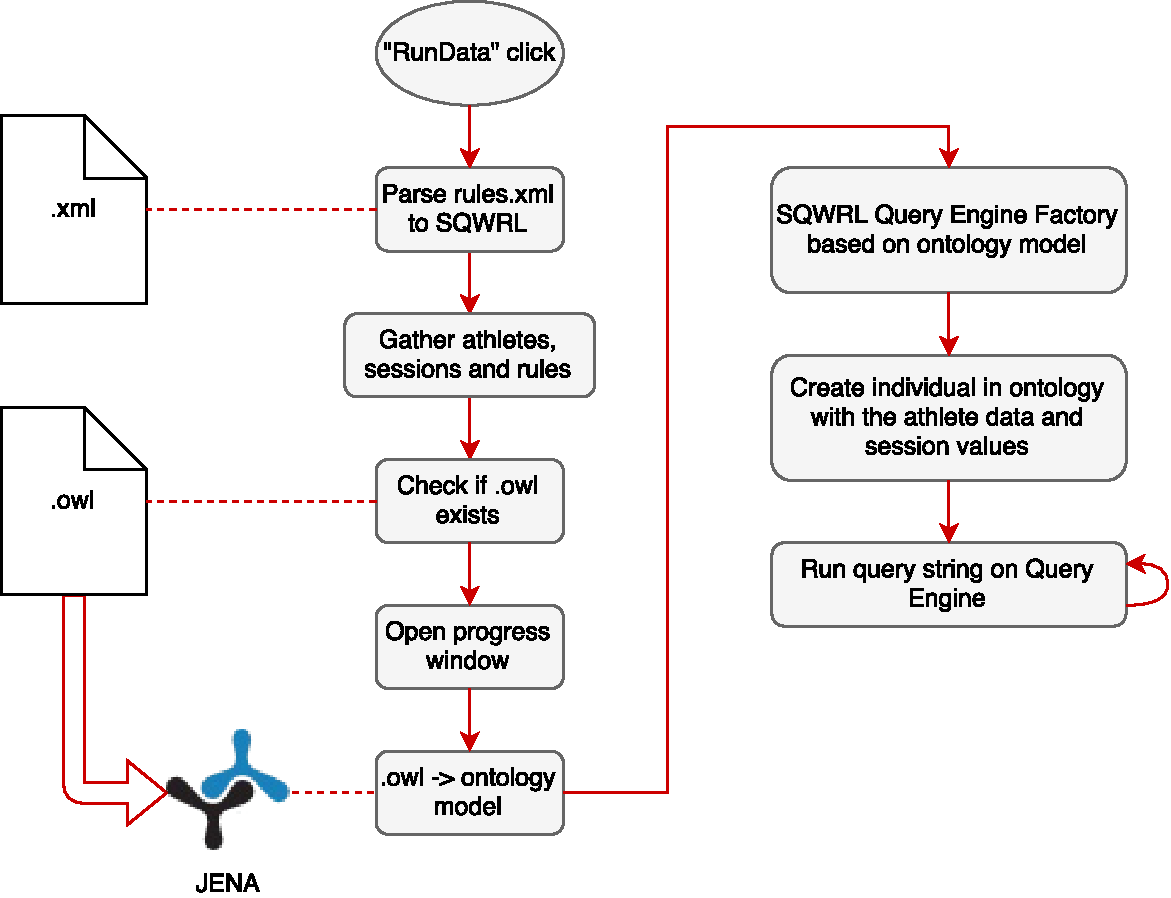
\includegraphics[width=1.00\textwidth]{Images/integration.pdf}
	\caption{Ontology integration.}
	\label{fig:ont_int}
\end{figure}

The selected API provides some methods that make the integration more easy.
The \textit{createJenaOWLModelFromURI()} method performs the construction of an OntModel from an OWLModel.
There is also the \textit{create()} method that is called on a \textbf{P3SQWRLQueryEngineFactory} object to create the query engine and this has the \textit{runSQWRLQuery()} method that is used to execute the queries and return the result. 


\newpage

%----------------------------------------------------------------------------------------%
% Conclusion
%----------------------------------------------------------------------------------------%
\section{Conclusion}
\input{texts/Conclusion.tex}
\newpage
%\bibliographystyle{abbrv}
\bibliographystyle{IEEEtran}
\nocite{*}
\bibliography{texts/bibliography}


\end{document}
